\chapter{Mezcla, oscilación, momentos dipolares eléctricos y operadores de campo}

Empezaremos apartándonos un poco del tema anunciado, con una pregunta sobre los neutrinos. Hay indicios de que los neutrinos tienen masa y de que sus tipos se mezclan. Si sus masas no son todas iguales, ¿cómo puede un tipo convertirse en otro sin violar la conservación de la energía?

La pregunta apunta a un patrón que aparece en toda la mecánica cuántica: los estados en los que se prepara o detecta un sistema no tienen por qué ser los que diagonalizan su hamiltoniano. Un estado de energía definida solo adquiere una fase. Un estado preparado como superposición de varias energías cambia porque sus componentes adquieren fases distintas. Esta distinción nos llevará de un pozo doble a la oscilación de neutrinos y la precesión del espín. Tras una digresión sobre el momento dipolar eléctrico del electrón, volveremos a la segunda cuantización y veremos la misma estructura de Fourier posición--momento en el nivel de los operadores.

\section{La mezcla como cuestión fundamental}

No es necesario que todos los neutrinos tengan la misma masa. Los estados propios de energía no se mezclan entre sí; cada uno evoluciona de manera independiente. Lo que llamamos \emph{tipo} o sabor de un neutrino está relacionado con la forma en que se produce y se detecta, y un estado de sabor puede ser una combinación lineal de estados propios de masa y energía. Esquemáticamente,
\begin{equation}
|\text{type}\rangle = \sum_n c_n |E_n\rangle .
\end{equation}
Así que lo correcto no es decir que los estados propios de energía se transforman unos en otros, sino que los estados llamados ``neutrino electrónico'' o ``neutrino muónico'' no tienen por qué ser, ellos mismos, estados propios de energía.

\begin{classroomqa}
\lecturetimestamp{00:00:09}
\audiencequestion{Si los neutrinos tienen masas distintas, ¿cómo pueden mezclarse y conservarse la energía?}
\lecturerresponse{Los estados propios de masa y energía no se transforman unos en otros. Los estados de sabor electrónico, muónico y tauónico son combinaciones lineales distintas de esos estados propios. Cada componente de masa evoluciona con su propia fase, y la interferencia modifica las probabilidades de sabor sin violar la conservación de la energía.}
\end{classroomqa}

Hay muchos ejemplos de esta estructura. El más visible comienza con una partícula en un pozo doble simétrico.

\section{Pozo doble simétrico y estados localizados aproximados}

Consideremos una partícula que se mueve en un potencial de doble pozo simétrico, con una barrera alta entre los dos mínimos. Si la barrera fuera infinitamente alta, los pozos izquierdo y derecho quedarían completamente desacoplados. Podríamos resolver el pozo de la izquierda como si el de la derecha no existiera, y viceversa. Las funciones de onda aproximadas del estado fundamental serían entonces un estado localizado a la izquierda \(\psi_L\) y otro localizado a la derecha \(\psi_R\), ambos con la misma energía \(E\).

En cada pozo aislado, el estado fundamental tiene las propiedades cualitativas habituales: es suave, no tiene nodos y se encuentra en la energía más baja posible compatible con el confinamiento. Pensemos en la alta barrera central como si fuera un muro de ladrillos. Considerarla infinita es solo una aproximación, pero nos proporciona un par útil de estados localizados como punto de partida.

\begin{figure}
\centering
\begin{adjustbox}{max width=\linewidth}
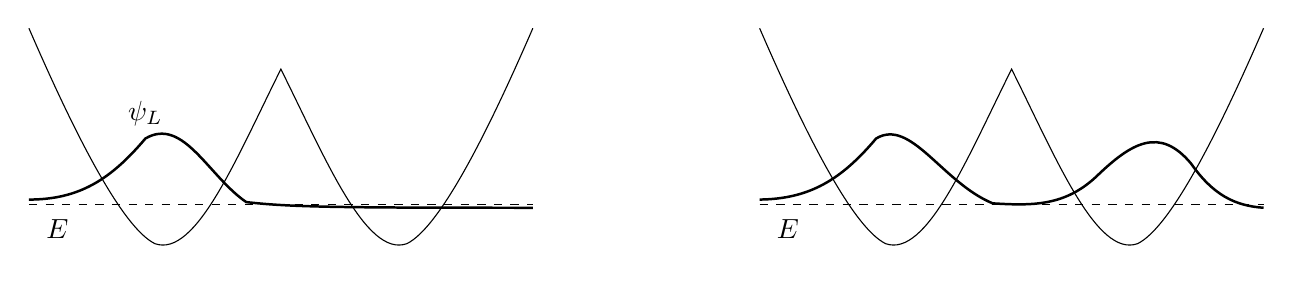
\begin{tikzpicture}[x=0.8cm,y=0.8cm]
\begin{scope}[shift={(-5.8,0)}]
\draw (-4,2.7) .. controls (-3.35,1.2) and (-2.55,-0.45) .. (-2.0,-0.72)
      .. controls (-1.35,-0.95) and (-0.7,0.65) .. (0,2.05)
      .. controls (0.7,0.65) and (1.35,-0.95) .. (2.0,-0.72)
      .. controls (2.55,-0.45) and (3.35,1.2) .. (4,2.7);
\draw[dashed] (-4,-0.10) -- (4,-0.10);
\node at (-3.55,-0.48) {$E$};
\draw[line width=0.9pt] (-4,-0.02) .. controls (-3.2,-0.02) and (-2.7,0.30) .. (-2.15,0.95)
      .. controls (-1.55,1.30) and (-1.15,0.35) .. (-0.55,-0.06)
      .. controls (0.15,-0.14) and (0.9,-0.15) .. (4,-0.15);
\node at (-2.15,1.35) {$\psi_L$};
\end{scope}
\begin{scope}[shift={(5.8,0)}]
\draw (-4,2.7) .. controls (-3.35,1.2) and (-2.55,-0.45) .. (-2.0,-0.72)
      .. controls (-1.35,-0.95) and (-0.7,0.65) .. (0,2.05)
      .. controls (0.7,0.65) and (1.35,-0.95) .. (2.0,-0.72)
      .. controls (2.55,-0.45) and (3.35,1.2) .. (4,2.7);
\draw[dashed] (-4,-0.10) -- (4,-0.10);
\node at (-3.55,-0.48) {$E$};
\draw[line width=0.9pt] (-4,-0.02) .. controls (-3.2,-0.01) and (-2.7,0.30) .. (-2.15,0.95)
      .. controls (-1.6,1.28) and (-1.1,0.25) .. (-0.30,-0.08)
      .. controls (0.35,-0.12) and (0.85,-0.12) .. (1.35,0.35)
      .. controls (1.9,0.88) and (2.35,1.15) .. (2.85,0.55)
      .. controls (3.2,0.05) and (3.55,-0.12) .. (4,-0.15);
\end{scope}
\end{tikzpicture}
\end{adjustbox}
\caption{Redibujo limpio de los primeros esquemas de la pizarra. A la izquierda está el estado de prueba unilateral \(\psi_L\), obtenido al suponer que la barrera es efectivamente infinita. A la derecha, la misma función de onda se prolonga simétricamente a través de la barrera, lo que ilustra la fuga pequeña pero no nula que acaba dando lugar al verdadero estado fundamental par.}
\end{figure}

Sin embargo, en mecánica cuántica la barrera no es realmente infinita. La función de onda en la región de la barrera no es exactamente cero; solo es muy pequeña. Toda la cuestión reside en esta fuga diminuta. Es lo que convierte la aproximación de izquierda y derecha en un verdadero problema de mezcla.

\section{Estados propios de paridad y desdoblamiento exponencial de niveles}

Ahora la imagen localizada queda interrumpida por un teorema: si el potencial es simétrico, las funciones propias exactas de la energía pueden elegirse simétricas o antisimétricas bajo reflexión.

\begin{theorem}
Si \(V(x)=V(-x)\) en una dimensión, las funciones propias del hamiltoniano pueden elegirse de modo que satisfagan una de estas dos condiciones:
\[
\psi(x)=\psi(-x)
\qquad \text{or} \qquad
\psi(x)=-\psi(-x).
\]
\end{theorem}

Ahora viene la corrección. Los estados unilaterales \(\psi_L\) y \(\psi_R\) no son ni simétricos ni antisimétricos, así que no pueden ser estados propios exactos del hamiltoniano completo. Solo son buenos estados aproximados cuando la barrera es alta. Los verdaderos estados propios son las combinaciones simétrica y antisimétrica,
\begin{align}
\psi_+ &= \frac{\psi_L+\psi_R}{\sqrt{2}},\\
\psi_- &= \frac{\psi_L-\psi_R}{\sqrt{2}}.
\end{align}
Con la notación que dejaremos en la pizarra, llamemos a sus energías
\begin{align}
H\psi_+ &= (E_1-\epsilon)\psi_+,\\
H\psi_- &= (E_1+\epsilon)\psi_-.
\end{align}
Por tanto, el desdoblamiento total es
\begin{equation}
\Delta E = (E_1+\epsilon)-(E_1-\epsilon)=2\epsilon .
\end{equation}

\begin{figure}[htbp]
\centering
\includegraphics[width=0.92\linewidth]{lecture_08_frame_02.png}
\caption{La función de onda prolongada simétricamente en el potencial de doble pozo. Su amplitud bajo la barrera es pequeña, pero no nula; de ahí se origina el desdoblamiento de niveles.}
\lectureframe{00:06:19}
\end{figure}

\begin{figure}
\centering
\begin{tikzpicture}[x=1cm,y=1cm]
\draw[->] (0,0) -- (0,3);
\node[left] at (0,2.8) {energy};
\draw (-0.35,1.60) -- (0.35,1.60);
\node[left] at (-0.45,1.60) {$\psi_L,\psi_R$};
\node at (1.7,1.60) {$\Longrightarrow$};
\draw (3.0,1.32) -- (3.75,1.32);
\draw (3.0,1.88) -- (3.75,1.88);
\draw[dashed] (2.8,1.60) -- (3.95,1.60);
\node[right] at (3.9,1.32) {$\psi_+,\ E_1-\epsilon$};
\node[right] at (3.9,1.88) {$\psi_-,\ E_1+\epsilon$};
\node[below] at (3.37,1.60) {$E_1$};
\end{tikzpicture}
\caption{El razonamiento de la pizarra sobre el desdoblamiento por efecto túnel. Los estados aproximados de izquierda y derecha son casi degenerados, pero los estados propios exactos, simétrico y antisimétrico, están separados por una pequeña cantidad \(2\epsilon\).}
\end{figure}

El orden de los niveles encierra el contenido físico. El estado simétrico tiene una energía ligeramente menor porque es más suave en la región de la barrera; permitir que la función de onda se filtre y continúe simétricamente reduce la energía en una cantidad diminuta. El estado antisimétrico tiene una energía ligeramente mayor porque el primer estado excitado en una dimensión tiene un nodo y, en este problema simétrico, ese nodo está en el punto medio. La curvatura adicional cuesta energía cinética.

El efecto es muy pequeño, exponencialmente pequeño en la anchura y la altura de la barrera. Aquí no necesitamos una fórmula explícita de WKB; lo importante es que el desdoblamiento es real, aunque diminuto. Recordemos también que el signo global de una función de onda no contiene información física. Sustituir \(\psi_-\) por \(-\psi_-\) no cambia el estado.

\section{Evolución temporal y oscilación entre izquierda y derecha}

Planteemos ahora la pregunta dinámica: ¿qué ocurre si colocamos una partícula en el pozo de la izquierda? Este es el paso decisivo, porque la oscilación es la manifestación temporal del mismo fenómeno de mezcla.

Las relaciones inversas son
\begin{align}
\psi_L &= \frac{\psi_+ + \psi_-}{\sqrt{2}},\\
\psi_R &= \frac{\psi_+ - \psi_-}{\sqrt{2}}.
\end{align}
Así, un estado inicialmente localizado a la izquierda es
\begin{equation}
\psi(0)=\psi_L=\frac{\psi_+ + \psi_-}{\sqrt{2}}.
\end{equation}
No es un estado propio de energía y, por tanto, debe evolucionar de manera no trivial.

Usamos la convención estándar de Schr\"odinger \(e^{-iEt}\). Una fase común no tiene efectos observables; solo la fase relativa entre los dos componentes de energía puede trasladar probabilidad de un pozo al otro.

Con esa convención,
\begin{equation}
\psi(t)=\frac{1}{\sqrt{2}}\left(e^{-i(E_1-\epsilon)t}\psi_+ + e^{-i(E_1+\epsilon)t}\psi_-\right).
\end{equation}
Esta es la versión depurada de la fórmula de la pizarra. Ahora saquemos factor común de la fase:
\begin{equation}
\psi(t)=\frac{e^{-iE_1 t}}{\sqrt{2}}\left(e^{i\epsilon t}\psi_+ + e^{-i\epsilon t}\psi_-\right).
\end{equation}
Una fase gira ahora en un sentido alrededor del círculo unidad y la otra en el sentido opuesto. El estado solo cambia porque estas dos fases se desfasan.

Para ver explícitamente la oscilación entre izquierda y derecha, sustituyamos las definiciones de \(\psi_\pm\):
\begin{align}
\psi(t)
&= \frac{e^{-iE_1 t}}{2}
\left[e^{i\epsilon t}(\psi_L+\psi_R)+e^{-i\epsilon t}(\psi_L-\psi_R)\right] \\
&= \frac{e^{-iE_1 t}}{2}
\left[(e^{i\epsilon t}+e^{-i\epsilon t})\psi_L+(e^{i\epsilon t}-e^{-i\epsilon t})\psi_R\right] \\
&= e^{-iE_1 t}\left[\psi_L\cos(\epsilon t)+i\,\psi_R\sin(\epsilon t)\right].
\end{align}
Esta es la derivación desarrollada clave del capítulo. En la aproximación de dos estados, con \(\psi_L\) y \(\psi_R\) ortonormales, las probabilidades son
\begin{equation}
P_L(t)=\cos^2(\epsilon t),
\qquad
P_R(t)=\sin^2(\epsilon t).
\end{equation}
Así que el sistema oscila. En los tiempos intermedios está realmente en una superposición; por ejemplo, cuando \(\epsilon t=\pi/4\), las probabilidades a ambos lados son iguales. Las fases evolucionan continuamente, y la localización cambia con ellas de manera continua.

La derivación en la pizarra aísla el primer instante en que cambia el signo relativo. Preguntamos cuándo se cumple
\begin{equation}
e^{-i\epsilon t}=-\,e^{i\epsilon t},
\end{equation}
que es el hito que se destaca en la pizarra. Al multiplicar ambos lados se obtiene
\begin{equation}
e^{2i\epsilon t}=-1.
\end{equation}
Para la primera vez que ocurre,
\begin{equation}
2\epsilon t=\pi,
\qquad\text{so}\qquad
t_{L\to R}=\frac{\pi}{2\epsilon}.
\end{equation}

\begin{figure}[htbp]
\centering
\includegraphics[width=0.94\linewidth]{lecture_08_frame_05.png}
\caption{Cálculo de la fase relativa en la pizarra. Los dos componentes de energía se vuelven opuestos cuando \(e^{2i\epsilon t}=-1\), lo que da el primer tiempo de transferencia \(2\epsilon t=\pi\). La derivación tipográfica emplea una sola convención de fase de Schr\"odinger.}
\lectureframe{00:17:52}
\end{figure}
En ese instante,
\begin{equation}
\psi(t_{L\to R}) \propto \frac{\psi_+-\psi_-}{\sqrt{2}}=\psi_R.
\end{equation}
La fase global es irrelevante. Lo que importa es que la partícula colocada inicialmente a la izquierda ha evolucionado hasta el estado localizado a la derecha. Tras otro intervalo igual, vuelve a oscilar hacia la izquierda. Mezcla y oscilación van juntas.

La ecuación no deja lugar a dudas: un valor pequeño de \(\epsilon\) implica oscilaciones lentas y un tiempo de transferencia largo. Ninguno de los dos estados localizados tiene energía definida, pero los dos componentes exactos de energía conservan la energía y evolucionan tal como deben.

\section{Analogías con neutrinos, amoníaco y espín}

El pozo doble nos proporciona un modelo para la pregunta original sobre los neutrinos. Un neutrino producido junto con un electrón se llama neutrino electrónico; uno producido junto con un muón se llama neutrino muónico. Esas etiquetas de sabor describen los canales de producción y detección. Los estados de masa definida y, por tanto, de energía definida para un momento fijo forman otra base.

En el modelo esquemático más sencillo de dos estados con mezcla máxima,
\begin{equation}
|\nu_e\rangle \sim \frac{|m_1\rangle+|m_2\rangle}{\sqrt{2}},
\qquad
|\nu_\mu\rangle \sim \frac{|m_1\rangle-|m_2\rangle}{\sqrt{2}},
\end{equation}
los estados propios de masa desempeñan el papel de \(\psi_+\) y \(\psi_-\), y los estados de sabor el de \(\psi_L\) y \(\psi_R\). La mezcla real de neutrinos utiliza una matriz de mezcla no trivial en lugar de estos coeficientes iguales, pero aquí ya se ve el mecanismo.

Un neutrino electrónico se produce en un proceso que involucra un electrón, igual que una partícula puede colocarse en el pozo de la izquierda. Durante un trayecto corto, sus dos componentes de masa acumulan fases casi iguales, por lo que una interacción todavía lo identifica como de sabor electrónico. A lo largo de una distancia grande, sus fases se separan. Entonces, una interacción posterior de corriente cargada puede producir un muón en vez de un electrón: el estado ha adquirido una componente de sabor muónico. Si se repite el experimento a distintas distancias o energías, se observa la oscilación.

No hay ningún conflicto con la conservación de la energía. Los estados propios de masa y energía hacen exactamente lo que deben hacer los estados propios. Lo que evoluciona es la superposición de sabores. En el límite relativista, la fase relativa observable está determinada por las diferencias de los cuadrados de las masas, esquemáticamente,
\begin{equation}
\Delta\phi_{ij}\simeq \frac{\Delta m_{ij}^{,2}L}{2E}.
\end{equation}
La oscilación muestra, por tanto, que no todas las masas de los neutrinos pueden ser idénticas: al menos dos estados propios de masa tienen masas distintas.

\begin{classroomqa}
\lecturetimestamp{00:24:06}
\audiencequestion{¿Qué determina el pequeño desdoblamiento \(\epsilon\) en el ejemplo del doble pozo?}
\lecturerresponse{Depende de la masa de la partícula y de la altura y anchura de la barrera. El efecto túnel es exponencialmente sensible a esos detalles, así que un cambio moderado en la barrera puede producir un gran cambio relativo en \(\epsilon\).}
\end{classroomqa}

\begin{classroomqa}
\lecturetimestamp{00:24:26}
\audiencequestion{¿Se ha observado realmente este fenómeno de oscilación?}
\lecturerresponse{Sí. Se observan desdoblamientos por efecto túnel en sistemas cuánticos ordinarios y oscilaciones de sabor en los neutrinos. Los mecanismos microscópicos son distintos, pero ambos realizan la misma evolución de fase en un sistema de dos estados.}
\end{classroomqa}

\begin{classroomqa}
\lecturetimestamp{00:24:34}
\audiencequestion{¿Qué relación hay entre la oscilación de neutrinos y la masa de los neutrinos?}
\lecturerresponse{Los estados propios que se propagan tienen masas distintas y, por tanto, acumulan fases distintas. Su interferencia modifica la composición de sabores. En un tratamiento relativista realista, lo que controla la oscilación son las diferencias de los cuadrados de las masas, no una masa de una partícula que varíe literalmente con el tiempo.}
\end{classroomqa}

\begin{classroomqa}
\lecturetimestamp{00:25:02}
\audiencequestion{¿La masa de los neutrinos es solo la teoría predominante o un hecho experimental?}
\lecturerresponse{La oscilación es un hecho experimental y requiere diferencias de masa distintas de cero. La escala absoluta de las masas es una magnitud distinta y más difícil de medir, pero los experimentos descartan la imagen mínima en la que todos los neutrinos carecen de masa.}
\end{classroomqa}

\subsection{Inversión del amoníaco: una barrera literal}

Una molécula de amoníaco, \(\mathrm{NH}_3\), tiene forma de pirámide trigonal: los tres átomos de hidrógeno forman un plano y el nitrógeno se encuentra a un lado de este. Existe una configuración equivalente con el nitrógeno al otro lado. Las dos configuraciones localizadas no son estados estacionarios exactos. El nitrógeno puede atravesar por efecto túnel el plano de hidrógeno, lo que produce estados propios de energía simétrico y antisimétrico y un pequeño desdoblamiento de inversión. Este es el origen físico de las mismas matemáticas en el máser de amoníaco.

\begin{classroomqa}
\lecturetimestamp{00:25:11}
\audiencequestion{En el amoníaco, ¿es la barrera la configuración en la que el nitrógeno atraviesa el plano de hidrógeno?}
\lecturerresponse{Sí. La energía molecular alcanza un mínimo en cualquiera de las dos configuraciones piramidales, mientras que la configuración plana tiene mayor energía. El efecto túnel a través de esta configuración acopla ambos lados.}
\end{classroomqa}

\begin{classroomqa}
\lecturetimestamp{00:27:10}
\audiencequestion{¿Cuál es la barrera física correspondiente entre los neutrinos electrónicos y muónicos?}
\lecturerresponse{No hay una barrera espacial literal. La analogía es algebraica: un acoplamiento no diagonal en el hamiltoniano de neutrinos mezcla la base de sabor. En el amoníaco, ese acoplamiento surge del efecto túnel; en los neutrinos, forma parte de la estructura de masas y mezcla.}
\end{classroomqa}

\subsection{Precesión del espín: mezcla sin efecto túnel}

Ya hemos encontrado el mismo álgebra en el espín. Tomemos los dos estados \(|\uparrow_z\rangle\) y \(|\downarrow_z\rangle\). Sin campo magnético son degenerados. Ahora apliquemos un campo magnético en la dirección \(x\). Los estados propios de energía ya no son los estados propios de \(z\), sino los estados polarizados en la dirección \(x\). Con los nombres provisionales izquierda--derecha de la pizarra,
\begin{align}
|L_x\rangle &= \frac{|\uparrow_z\rangle+|\downarrow_z\rangle}{\sqrt{2}},\\
|R_x\rangle &= \frac{|\uparrow_z\rangle-|\downarrow_z\rangle}{\sqrt{2}}.
\end{align}
Estos son los análogos directos de \(\psi_+\) y \(\psi_-\). El momento magnético alineado con el campo y el alineado en sentido opuesto tienen energías ligeramente distintas. Si esas energías son \(E\mp\epsilon\), un espín inicialmente hacia arriba evoluciona como sigue:
\begin{equation}
|\uparrow_z,t\rangle
= e^{-iEt}\left[\cos(\epsilon t)\,|\uparrow_z\rangle
+ i\sin(\epsilon t)\,|\downarrow_z\rangle\right].
\end{equation}
Esta es la misma fórmula que en el caso del doble pozo, solo que ahora la evolución continua corresponde a la precesión del espín alrededor del eje \(x\). Partiendo de \(+z\), el espín pasa por direcciones transversales, llega a \(-z\) tras medio período de precesión y vuelve después de otro medio período. Al medir \(S_z\) se obtiene todavía solo arriba o abajo; el estado de espín, que cambia continuamente, determina sus probabilidades. El mecanismo no requiere efecto túnel. Solo requiere que el hamiltoniano sea diagonal en una base distinta de la base de preparación.

\begin{classroomqa}
\lecturetimestamp{00:32:25}
\audiencequestion{¿Qué ocurre con el neutrino tauónico en este modelo?}
\lecturerresponse{También se mezcla. El problema real tiene tres estados de sabor y tres estados de masa, así que una matriz de mezcla de tres por tres reemplaza a la rotación de dos estados. El principio de interferencia de fases no cambia.}
\end{classroomqa}

\begin{classroomqa}
\lecturetimestamp{00:32:57}
\audiencequestion{Justo después de aplicar el campo transversal, ¿el espín sigue apuntando hacia arriba? ¿Puede orientarse hacia nosotros o en sentido opuesto?}
\lecturerresponse{Al cabo de un tiempo muy corto, sigue apuntando hacia arriba con una probabilidad casi segura, aunque existe una pequeña probabilidad de que apunte hacia abajo. El estado precesa continuamente alrededor del eje del campo y pasa por las direcciones transversales \(\pm y\), mientras permanece perpendicular al campo dirigido según \(x\) si inicialmente era perpendicular. Una medición a lo largo de cualquier eje elegido sigue dando uno de sus valores propios discretos.}
\end{classroomqa}

\begin{classroomqa}
\lecturetimestamp{00:34:30}
\audiencequestion{¿Se elige un campo débil para que el espín nunca apunte en la dirección del campo?}
\lecturerresponse{No. La geometría se debe a la precesión alrededor del eje del campo, no a que el campo sea débil. Un campo débil simplemente hace pequeña la separación de energía y la frecuencia de precesión, lo que produce una oscilación lenta análoga al ejemplo de los neutrinos.}
\end{classroomqa}

La intensidad de la mezcla de neutrinos y sus pequeñas masas son parámetros cuyo origen más profundo no explica el Modelo Estándar mínimo tal como se formuló originalmente. Por tanto, la masa de los neutrinos apunta más allá de ese modelo mínimo, aunque la escala observada es muy pequeña y podría reflejar física a una escala de energía muy remota.

\begin{classroomqa}
\lecturetimestamp{00:36:27}
\audiencequestion{¿Es la oscilación la razón por la que sabemos que los neutrinos tienen masa?}
\lecturerresponse{Es la prueba directa decisiva de que los componentes que se propagan tienen masas distintas. Si todos los componentes pertinentes fueran exactamente sin masa y degenerados, no acumularían ninguna fase relativa dependiente de la masa y no habría una oscilación de sabor en el vacío de este tipo.}
\end{classroomqa}

\begin{classroomqa}
\lecturetimestamp{00:37:57}
\audiencequestion{A mitad de un período, ¿debería un neutrino comportarse la mitad de las veces como de sabor electrónico y la otra mitad como de sabor muónico?}
\lecturerresponse{En el modelo ideal simétrico de dos estados, las probabilidades son iguales a un cuarto del período completo de probabilidad, mientras que la conversión completa ocurre en el primer máximo. Las oscilaciones reales de tres sabores tienen ángulos de mezcla desiguales, varias frecuencias, restricciones de espín y helicidad, y efectos de la materia, así que una conversión simétrica completa no es lo habitual.}
\end{classroomqa}

\begin{classroomqa}
\lecturetimestamp{00:38:36}
\audiencequestion{Si los componentes de masa son distintos, ¿debe cambiar la velocidad de un neutrino solar para conservar el momento?}
\lecturerresponse{Un estado de sabor es una superposición coherente de componentes de masas fijas; su masa no es una magnitud clásica que oscile con el tiempo. En la descripción habitual de momento igual, los componentes tienen energías y velocidades de grupo ligeramente distintas; en una descripción de energía igual, tienen momentos ligeramente distintos. Ambas convenciones dan la misma fase de oscilación observable si se tratan de manera coherente.}
\end{classroomqa}

Esta evolución de fase resolvió el antiguo déficit de neutrinos solares. Los primeros detectores eran sensibles principalmente a los neutrinos electrónicos, así que los neutrinos que salían del Sol como de sabor electrónico podían llegar en parte como muónicos o tauónicos y dejar de ser detectados en ese canal. El cálculo solar detallado incluye la mezcla de tres sabores y efectos de la materia, pero la lección conceptual ya está en el doble pozo: la preparación y la propagación utilizan bases distintas.

\section{Digresión: momento dipolar eléctrico, simetría y la afirmación de que el electrón es una ``esfera''}

Como ya estamos hablando de fenomenología de partículas, hagamos una pausa en las matemáticas formales. Un artículo divulgativo describió un nuevo límite para el momento dipolar eléctrico del electrón diciendo que se había demostrado que el electrón era una esfera. Ese eslogan confunde tres preguntas distintas: qué mide un momento dipolar eléctrico, qué significa la simetría rotacional para un estado cuántico y qué limitó realmente el experimento.

\subsection{¿Qué se midió?}

Lo que se midió —o, mejor dicho, se acotó— fue el momento dipolar eléctrico del electrón. Para cargas separadas \(\pm q\), el momento dipolar es
\begin{equation}
\mathbf d = q\,\boldsymbol{\ell},
\end{equation}
donde \(\boldsymbol{\ell}\) es el vector de separación. Un momento dipolar distinto de cero significa que la distribución de carga está desplazada respecto de cierto centro.

Para el electrón, sin embargo, la pregunta pertinente no es simplemente si la carga está descentrada en alguna dirección arbitraria. El electrón tiene espín y, por tanto, un eje. También tiene un momento magnético. La pregunta físicamente significativa es si existe una correlación entre el desplazamiento de la carga y ese eje:
\begin{equation}
\mathbf d_e \parallel \boldsymbol{\mu}_e
\qquad \text{or equivalently} \qquad
\mathbf d_e \parallel \mathbf S .
\end{equation}
A eso nos referimos con el momento dipolar eléctrico del electrón. Conceptualmente, nos preguntamos si, al colocar un electrón polarizado en espín en un campo eléctrico, se separan en energía las dos orientaciones del espín:
\begin{equation}
H_{\mathrm{EDM}}=-\mathbf d_e\cdot \mathbf E,
\qquad
\mathbf d_e=d_e\frac{\mathbf S}{|\mathbf S|}.
\end{equation}
El experimento real de sobremesa es mucho más sutil que un electrón desnudo entre las placas de un condensador, pero esta es la idea de simetría y cambio de energía que aprovecha.

\subsection{Por qué la ausencia de EDM no significa que sea una esfera}

La primera corrección es elemental. Un cuerpo puede no tener momento dipolar y aun así no ser esférico. Un elipsoide centrado tiene tanta carga a un lado como al otro y, por tanto, no tiene dipolo; sin embargo, puede tener un momento cuadrupolar. Una distribución aún más complicada puede carecer tanto de dipolo como de cuadrupolo y conservar un multipolo de orden superior. Medir un coeficiente multipolar no determina una forma completa.

La mecánica cuántica hace más delicada la palabra ``forma''. Imaginemos una molécula de dos átomos, parecida a una mancuerna, con una longitud de enlace aproximadamente fija. Ignoremos las vibraciones radiales y consideremos solo las rotaciones. Los estados rotacionales se etiquetan por el momento angular. Si la molécula es bosónica, el estado rotacional más bajo tiene \(J=0\). Como el momento angular genera las rotaciones,
\begin{equation}
\begin{gathered}
J=0 \quad\Longrightarrow\\
\text{rotationally invariant ground state.}
\end{gathered}
\end{equation}
El estado cuántico es invariante bajo rotaciones, aunque toda imagen con orientación definida parece una mancuerna. Puede describirse como una superposición coherente de todas las orientaciones. Llamar ``esférico'' al estado resulta útil para algunas mediciones y engañoso para otras.

Tomemos una instantánea. Una instantánea es una medición de la orientación, y una medición de orientación suficientemente precisa deja al sistema en un estado localizado en ángulo. Ese estado no puede tener también un momento angular definido. Esta es la versión rotacional del principio de incertidumbre posición--momento: localizar el ángulo necesariamente introduce una dispersión de momentos angulares y, por tanto, excitación rotacional.

Para un rotor rígido,
\begin{equation}
E_J=\frac{J(J+1)}{2I},
\end{equation}
por lo que la energía necesaria para resolver la estructura está determinada por el momento de inercia \(I\). Una mancuerna de gimnasio tiene un \(I\) enorme y niveles rotacionales extraordinariamente próximos; la luz ordinaria puede perturbarla con facilidad lo suficiente para revelar una orientación. En una molécula, la separación entre niveles es mayor. En un hadrón compacto, lo es aún más. Si la sonda no tiene energía suficiente para excitar la primera estructura rotacional resoluble, las mediciones repetidas solo ven el estado fundamental promediado sobre las rotaciones.

Un mesón puede imaginarse, de manera aproximada, como un sistema de dos cuerpos formado por un quark--antiquark. Sus primeras excitaciones orbitales cuestan cientos de millones de electronvoltios o más, muy por encima de la energía de un fotón óptico. Por tanto, una sonda de baja energía no puede tomar una instantánea de la orientación subyacente. ``Que sea una esfera o no'' depende en parte del estado preparado y en parte de la resolución del aparato.

El electrón precisa aún más la cuestión. Es una partícula de espín \(\tfrac12\), no un escalar rotacional. Un estado polarizado en espín tiene un eje y un momento magnético. La imagen habitual de una carga que circula alrededor de ese eje es solo una heurística---una partícula de Dirac puntual no es literalmente una pequeña esfera que gira---, pero nos recuerda correctamente que el momento magnético se invierte con el espín. La pregunta sobre el EDM es si el desplazamiento de carga eléctrica está correlacionado con ese mismo eje. Una respuesta nula no convierte al electrón en una esfera clásica.

\begin{classroomqa}
\lecturetimestamp{00:57:30}
\audiencequestion{¿El desplazamiento de parte de la carga del electrón violaría la cuantización de la carga?}
\lecturerresponse{No. La cuantización de la carga fija la carga total. El momento dipolar se refiere al primer momento espacial de esa distribución de carga o, de manera equivalente, a un acoplamiento permitido de una partícula puntual con el campo eléctrico; no requiere un cambio fraccionario de la carga total.}
\end{classroomqa}

\begin{classroomqa}
\lecturetimestamp{00:58:00}
\audiencequestion{¿Están prohibidos los momentos dipolares eléctricos por la teoría cuántica de campos?}
\lecturerresponse{La teoría cuántica de campos en sí no los prohíbe. Quedan prohibidos cuando ciertas simetrías discretas son exactas. Si se violan esas simetrías, se permite un operador EDM, aunque su coeficiente pueda ser extremadamente pequeño.}
\end{classroomqa}

\subsection{Paridad e inversión temporal}

El contenido real de la discusión sobre el EDM es la simetría. Bajo paridad, un momento dipolar eléctrico se transforma como un vector polar ordinario, mientras que un momento magnético se transforma como un vector axial:
\begin{align}
P:\qquad &\mathbf d_e \to -\mathbf d_e,
&\boldsymbol{\mu}_e \to \boldsymbol{\mu}_e .
\end{align}
Bajo inversión temporal, la corriente circulante que define el momento magnético se invierte, pero un desplazamiento electrostático no:
\begin{align}
T:\qquad &\mathbf d_e \to \mathbf d_e,
&\boldsymbol{\mu}_e \to -\boldsymbol{\mu}_e .
\end{align}
Por tanto, un EDM distinto de cero alineado con el eje de espín del electrón está prohibido si la simetría de paridad es exacta y también si la simetría de inversión temporal es exacta:
\begin{equation}
(P\ \text{exact}) \Rightarrow \mathbf d_e=0,
\qquad
(T\ \text{exact}) \Rightarrow \mathbf d_e=0.
\end{equation}

Conviene explicitar la geometría. Un momento magnético se produce mediante una corriente en forma de lazo. La reflexión especular invierte los vectores polares ordinarios, pero deja inalterado el vector axial normal a ese lazo. El desplazamiento de carga a lo largo del eje sí se invierte. Así, un electrón con \(\mathbf d_e\) paralelo a \(\boldsymbol\mu_e\) se transformaría por reflexión especular en uno con la misma orientación magnética, pero con la relación entre los momentos eléctrico y magnético invertida. Si la paridad fuera exacta y solo hubiera una especie de electrón, las dos descripciones tendrían que representar la misma partícula; solo \(d_e=0\) es compatible.

La inversión temporal lleva a la misma conclusión de otra manera. Al reproducir la película al revés, la corriente se invierte y, por tanto, también \(\boldsymbol\mu_e\), pero el desplazamiento estático de carga no cambia. Un estado con momentos paralelos pasa a ser uno con momentos antiparalelos. La simetría exacta bajo inversión temporal exigiría de nuevo \(d_e=0\).

\begin{figure}[htbp]
\centering
\begin{tikzpicture}[>=Stealth,scale=0.95]
  \node[font=\bfseries] at (1.0,2.25) {original};
  \draw[->,very thick,blue!70!black] (0.65,0) -- (0.65,1.65);
  \draw[->,very thick,red!75!black] (1.35,0) -- (1.35,1.65);
  \node[blue!70!black,below] at (0.65,0) {$\boldsymbol\mu$};
  \node[red!75!black,below] at (1.35,0) {$\mathbf d$};

  \node[font=\bfseries] at (4.5,2.25) {parity};
  \draw[->,very thick,blue!70!black] (4.15,0) -- (4.15,1.65);
  \draw[->,very thick,red!75!black] (4.85,1.65) -- (4.85,0);
  \node[blue!70!black,below] at (4.15,0) {$\boldsymbol\mu$};
  \node[red!75!black,below] at (4.85,0) {$-\mathbf d$};

  \node[font=\bfseries] at (8.0,2.25) {time reversal};
  \draw[->,very thick,blue!70!black] (7.65,1.65) -- (7.65,0);
  \draw[->,very thick,red!75!black] (8.35,0) -- (8.35,1.65);
  \node[blue!70!black,below] at (7.65,0) {$-\boldsymbol\mu$};
  \node[red!75!black,below] at (8.35,0) {$\mathbf d$};
\end{tikzpicture}
\caption{La prueba de simetría reconstruida a partir del argumento en la pizarra. La paridad invierte el dipolo eléctrico, pero no el momento magnético axial; la inversión temporal invierte el momento magnético, pero no el desplazamiento eléctrico estático. Si cualquiera de estas simetrías fuera exacta, prohibiría un EDM permanente paralelo al espín.}
\end{figure}

\begin{figure}[htbp]
\centering
\includegraphics[width=0.94\linewidth]{lecture_08_frame_06.png}
\caption{Los esquemas emparejados del eje magnético y el desplazamiento de carga durante el argumento sobre la inversión temporal. El diagrama compacto en TikZ de arriba aísla el contenido de las transformaciones de la pizarra original, parcialmente borrada.}
\lectureframe{01:06:10}
\end{figure}

\begin{classroomqa}
\lecturetimestamp{01:06:38}
\audiencequestion{Bajo inversión temporal, ¿se invierten tanto las corrientes como las cargas?}
\lecturerresponse{Las corrientes se invierten porque las velocidades se invierten; la carga eléctrica en sí no. La conjugación de carga \(C\), y no la inversión temporal \(T\), invierte el signo de la carga.}
\end{classroomqa}

\begin{classroomqa}
\lecturetimestamp{01:07:01}
\audiencequestion{¿El carácter antiunitario de la inversión temporal significa que la mecánica cuántica no relativista no es invariante bajo inversión temporal?}
\lecturerresponse{No. La antiunitariedad es precisamente la forma de representar la inversión temporal de manera coherente en mecánica cuántica: conjuga complejamente las amplitudes e invierte los momentos y los espines. Que un Hamiltoniano particular sea invariante es una cuestión distinta.}
\end{classroomqa}

\begin{classroomqa}
\lecturetimestamp{01:07:19}
\audiencequestion{¿Para hablar de un EDM es necesario que el electrón tenga un volumen finito, en vez de ser puntual?}
\lecturerresponse{No. Un Hamiltoniano efectivo para una partícula puntual puede contener \(-d_e\,\widehat{\mathbf S}\!\cdot\!\mathbf E\). El experimento pregunta si orientaciones opuestas del espín adquieren energías distintas en un campo eléctrico; no es necesario resolver una nube de carga extensa literal.}
\end{classroomqa}

La paridad no es una simetría de las interacciones débiles; se viola al máximo en sus acoplamientos quirales. La inversión temporal tampoco es exacta, pero la violación conocida en el Modelo Estándar contribuye al EDM del electrón solo a un nivel extraordinariamente pequeño. Se puede calcular una contribución no nula del Modelo Estándar, pero queda muy por debajo de la sensibilidad de la que hablamos aquí. Por tanto, un resultado nulo es compatible con el Modelo Estándar, aunque restringe extensiones---la supersimetría y otras interacciones nuevas, por ejemplo---que pueden generar una violación de la inversión temporal mucho mayor.

La idea experimental básica es sencilla. Un campo magnético revela un dipolo magnético al separar las orientaciones del espín. Un campo eléctrico revelaría un EDM mediante un desplazamiento adicional de la energía correlacionado con el espín. Los experimentos de precisión reales emplean átomos o moléculas, largos tiempos de precesión coherente, inversiones de los campos aplicados y un control cuidadoso de los efectos sistemáticos, en vez de un electrón aislado en un dispositivo ingenuo.

\begin{classroomqa}
\lecturetimestamp{01:11:02}
\audiencequestion{¿La búsqueda del EDM fue un experimento de colisiones de alta energía o un experimento con objetos materiales?}
\lecturerresponse{Fue un experimento de precisión de sobremesa, con electrones ligados en un entorno atómico o molecular controlado, junto con campos eléctricos y magnéticos. Su energía es baja, pero su sensibilidad a desplazamientos minúsculos que violan simetrías permite sondear indirectamente nueva física de alta energía.}
\end{classroomqa}

\begin{classroomqa}
\lecturetimestamp{01:12:21}
\audiencequestion{¿El resultado nulo restringe cuáles modificaciones del Modelo Estándar siguen siendo viables?}
\lecturerresponse{Sí, en principio: cada modelo predice un coeficiente y, por tanto, ocupa cierta región de parámetros. La exclusión numérica detallada requiere un cálculo especializado, pero la lógica general es firme---cuanto mayor es la precisión con que concuerdan los resultados con el Modelo Estándar, menos margen queda para alternativas que predigan un EDM grande.}
\end{classroomqa}

\begin{classroomqa}
\lecturetimestamp{01:13:09}
\audiencequestion{¿Se requiere la simetría bajo inversión temporal para conservar la información cuántica?}
\lecturerresponse{No. La evolución temporal unitaria conserva la información incluso cuando un Hamiltoniano no es invariante bajo \(T\). Una partícula en un campo magnético fijo es un ejemplo conocido: el campo selecciona una orientación en las películas invertidas temporalmente, a menos que también se invierta el campo, pero la evolución cuántica sigue siendo unitaria. Bajo las hipótesis habituales de la teoría cuántica de campos local e invariante de Lorentz, la transformación combinada \(CPT\) es una simetría, pero eso no es lo que garantiza la unitariedad.}
\end{classroomqa}

El descanso puede terminar ahora. La medición nula indica que no se ha detectado ningún EDM del electrón con la sensibilidad indicada. No afirma que el electrón sea una esfera ni refuta el Modelo Estándar; hace más difícil sostener algunas desviaciones propuestas respecto de ese modelo.

\section{Regreso a la segunda cuantización: transformadas de Fourier, modos de momento y localidad}

Estábamos estudiando la segunda cuantización. Empecemos de nuevo con calma, a partir de un hecho conocido sobre las funciones de onda ordinarias de una partícula, y luego extendámoslo a los operadores. La conexión con las transformadas de Fourier es exacta y sencilla.

\subsection{Del espacio de posiciones al espacio de momentos}

La letra minúscula \(\psi\), no la mayúscula \(\Psi\), representa la función de onda de una sola partícula. En el espacio de posiciones,
\begin{equation}
P(x)=|\psi(x)|^2
\end{equation}
es la densidad de probabilidad de encontrar la partícula en la posición \(x\). La función de onda en el espacio de momentos es su transformada de Fourier,
\begin{equation}
\tilde{\psi}(p)=\int dx\,\psi(x)\,\frac{e^{-ipx}}{\sqrt{2\pi}},
\end{equation}
y la relación inversa es
\begin{equation}
\psi(x)=\int dp\,\tilde{\psi}(p)\,\frac{e^{ipx}}{\sqrt{2\pi}}.
\end{equation}
Entonces,
\begin{equation}
P(p)=|\tilde{\psi}(p)|^2
\end{equation}
es la densidad de probabilidad del momento \(p\).

Usamos \(\hbar=1\). Las dos transformadas son inversas: conocer cualquiera de las dos funciones de onda determina la otra, mientras que sus módulos al cuadrado responden a preguntas de medición distintas.

Para una partícula libre,
\begin{equation}
H=\frac{p^2}{2m},
\end{equation}
por lo que los estados propios del momento también son estados propios de la energía, y sus funciones de onda en el espacio de posiciones son ondas planas,
\begin{equation}
\psi_p(x)\propto e^{ipx}.
\end{equation}
Este es el punto de partida para la versión en segunda cuantización.

\begin{figure}[htbp]
\centering
\includegraphics[width=0.94\linewidth]{lecture_08_frame_07.png}
\caption{Par de Fourier entre posición--momento para una función de onda de una partícula. Es esencial distinguir \(\psi\) del operador de campo, que se introduce a continuación.}
\lectureframe{01:20:00}
\end{figure}

\subsection{Operadores de campo en los espacios de posiciones y de momentos}

Volvamos ahora al operador de campo. En la pizarra, sus partes de aniquilación y creación se escriben como \(\Psi_-(x)\) y \(\Psi_+(x)\). Manteniendo por un momento esa notación,
\begin{align}
\Psi_-(x) &= \sum_i a_i\,\psi_i(x),\\
\Psi_+(x) &= \sum_i a_i^\dagger\,\psi_i^*(x).
\end{align}
Aquí, \(\psi_i(x)\) es la función de onda ordinaria de una partícula para el modo \(i\), mientras que \(a_i\) y \(a_i^\dagger\) aniquilan y crean partículas en ese modo. A partir de aquí conviene cambiar la notación a
\[
\Psi(x)\equiv \Psi_-(x),
\qquad
\Psi^\dagger(x)\equiv \Psi_+(x).
\]

Para una partícula libre, la etiqueta discreta del modo \(i\) se sustituye por la etiqueta continua del momento \(p\). Usando las ondas planas \(e^{ipx}\), se obtienen las fórmulas reconstruidas habituales
\begin{align}
\Psi(x) &= \int \frac{dp}{\sqrt{2\pi}}\,a(p)\,e^{ipx},\\
\Psi^\dagger(x) &= \int \frac{dp}{\sqrt{2\pi}}\,a^\dagger(p)\,e^{-ipx}.
\end{align}
Estas son las fórmulas análogas a la transformada de Fourier ordinaria para los operadores de campo. Se pueden invertir exactamente como antes:
\begin{align}
a(p) &= \int \frac{dx}{\sqrt{2\pi}}\,\Psi(x)\,e^{-ipx},\\
a^\dagger(p) &= \int \frac{dx}{\sqrt{2\pi}}\,\Psi^\dagger(x)\,e^{ipx}.
\end{align}
Los factores de \(1/\sqrt{2\pi}\) son una convención elegida para que las transformadas directa e inversa tengan la misma normalización.

El contenido conceptual es sencillo. \(\Psi^\dagger(x)\) crea una partícula en la posición \(x\), mientras que \(a^\dagger(p)\) crea una partícula con momento \(p\). Los operadores de creación en los espacios de posiciones y de momentos son conjugados de Fourier entre sí, igual que \(\psi(x)\) y \(\tilde{\psi}(p)\) lo son en la mecánica cuántica ordinaria.

Si no hay ninguna partícula con momento \(p\), \(a(p)\) aniquila el estado. Si hay partículas con ese momento, elimina una con el coeficiente habitual del número de ocupación. Del mismo modo, \(\Psi(x)\) elimina una partícula en \(x\), entendido en el sentido de distribuciones o tras integrar el campo para formar un paquete de ondas. Cada especie de partícula requiere su propio operador de campo; un único campo no puede crear todas las clases de partículas.

\subsection{Conmutadores bosónicos e independencia de las mediciones en regiones separadas}

El siguiente resultado se deduce directamente de las definiciones. Para los bosones,
\begin{equation}
[a_i,a_j^\dagger]=\delta_{ij},
\qquad
[a_i,a_j]=0,
\qquad
[a_i^\dagger,a_j^\dagger]=0.
\end{equation}
La versión continua es
\begin{equation}
[a(p),a^\dagger(p')]=\delta(p-p').
\end{equation}
Calculemos ahora el conmutador de los campos a tiempos iguales a partir de la expansión discreta:
\begin{align}
[\Psi(x),\Psi^\dagger(y)]
&= \sum_{i,j}\psi_i(x)\psi_j^*(y)\,[a_i,a_j^\dagger] \\
&= \sum_i \psi_i(x)\psi_i^*(y) \\
&= \delta(x-y),
\end{align}
donde el último paso usa la completitud de la base de una partícula. Asimismo,
\begin{equation}
[\Psi(x),\Psi(y)]=0,
\qquad
[\Psi^\dagger(x),\Psi^\dagger(y)]=0.
\end{equation}

\begin{figure}[htbp]
\centering
\includegraphics[width=0.94\linewidth]{lecture_08_frame_08.png}
\caption{El conmutador de los modos y su correspondiente en el espacio de posiciones, tal como aparecen en la pizarra. La completitud convierte \(\delta_{ij}\) en la distribución delta espacial \(\delta(x-y)\).}
\lectureframe{01:31:00}
\end{figure}

Lo importante no es solo que \(\Psi\) no sea hermítico. Definamos las cuadraturas hermíticas
\begin{equation}
Q(x)=\frac{\Psi(x)+\Psi^\dagger(x)}{\sqrt{2}},
\qquad
P(x)=\frac{\Psi(x)-\Psi^\dagger(x)}{i\sqrt{2}}.
\end{equation}
Su conmutador en un mismo punto hereda la distribución delta. Así, las dos cuadraturas locales son conjugadas en el mismo sentido en que lo son la posición y el momento. Intentar precisar una aumenta la incertidumbre de la otra.

\begin{classroomqa}
\lecturetimestamp{01:32:03}
\audiencequestion{¿Qué significa la función delta cuando \(x=y\)? ¿Es grande el conmutador en todas partes?}
\lecturerresponse{La delta es una distribución, no una función ordinaria con un valor finito en cada punto. Se anula para argumentos separados y solo da un resultado finito al integrarla contra una función de prueba. Al integrar los campos sobre una región finita del detector, la singularidad formal en un mismo punto se convierte en el conmutador canónico finito habitual de dos modos.}
\end{classroomqa}

Sin embargo, para \(x\neq y\), el conmutador a tiempos iguales se anula. Las operaciones localizadas en dos regiones disjuntas pueden realizarse de forma independiente: medir el campo aquí no da una sacudida cuántica al campo allí. Este es el antecedente no relativista, a tiempos iguales, de la microcausalidad relativista. En una teoría relativista, los observables locales físicos conmutan cuando están separados espacialmente, pues ninguna señal luminosa puede conectar los dos eventos.

El contraste con los observables que no conmutan es conocido. Como \([x,p]=i\), una medición precisa de la posición perturba el momento, y un estado con momento preciso se dispersa en posición. Como las distintas componentes del espín no conmutan, preparar una de ellas con precisión hace que otra sea incierta. Un conmutador no nulo entre observables locales separados significaría, de manera análoga, que una operación en una región perturba la otra, en contradicción con la independencia causal requerida.

\begin{classroomqa}
\lecturetimestamp{01:37:51}
\audiencequestion{¿Los experimentos EPR y de entrelazamiento demuestran que una medición aquí afecta a una medición distante?}
\lecturerresponse{Demuestran que hay correlaciones, no una influencia causal controlable. Los resultados entrelazados violan la factorización clásica, pero no se pueden cambiar las estadísticas locales del detector distante eligiendo o realizando aquí una medición. La conmutación de observables separados espacialmente es la formulación en términos de operadores de esa independencia que impide la señalización.}
\end{classroomqa}

La próxima vez cambiará el álgebra. Los operadores de creación y aniquilación de fermiones satisfacen relaciones de anticonmutación. Tomado al pie de la letra, los campos fermiónicos en puntos separados no conmutan, de modo que los propios campos no pueden interpretarse directamente como observables bosónicos medibles. Los observables fermiónicos físicos son combinaciones pares---densidades, corrientes, tensores de energía-momento---y esos observables locales recuperan la conmutatividad requerida para separaciones espaciales. Ese es el punto de partida para la versión fermiónica de la segunda cuantización.
